\documentclass{ximera}  


%\usepackage{todonotes}
%\usepackage{mathtools} %% Required for wide table Curl and Greens
%\usepackage{cuted} %% Required for wide table Curl and Greens
\newcommand{\todo}{}

\usepackage{esint} % for \oiint
\ifxake%%https://math.meta.stackexchange.com/questions/9973/how-do-you-render-a-closed-surface-double-integral
\renewcommand{\oiint}{{\large\bigcirc}\kern-1.56em\iint}
\fi


\graphicspath{
  {./}
  {jpg}
  {ximeraTutorial/}
  {basicPhilosophy/}
  {functionsOfSeveralVariables/}
  {normalVectors/}
  {lagrangeMultipliers/}
  {vectorFields/}
  {greensTheorem/}
  {shapeOfThingsToCome/}
  {dotProducts/}
  {partialDerivativesAndTheGradientVector/}
  {../productAndQuotientRules/exercises/}
  {../motionAndPathsInSpace/exercises/}
  {../normalVectors/exercisesParametricPlots/}
  {../continuityOfFunctionsOfSeveralVariables/exercises/}
  {../partialDerivativesAndTheGradientVector/exercises/}
  {../directionalDerivativeAndChainRule/exercises/}
  {../commonCoordinates/exercisesCylindricalCoordinates/}
  {../commonCoordinates/exercisesSphericalCoordinates/}
  {../greensTheorem/exercisesCurlAndLineIntegrals/}
  {../greensTheorem/exercisesDivergenceAndLineIntegrals/}
  {../shapeOfThingsToCome/exercisesDivergenceTheorem/}
  {../greensTheorem/}
  {../shapeOfThingsToCome/}
  {../separableDifferentialEquations/exercises/}
  {vectorFields/}
}

\newcommand{\mooculus}{\textsf{\textbf{MOOC}\textnormal{\textsf{ULUS}}}}

\usepackage{tkz-euclide}\usepackage{tikz}
\usepackage{tikz-cd}
\usetikzlibrary{arrows}
\tikzset{>=stealth,commutative diagrams/.cd,
  arrow style=tikz,diagrams={>=stealth}} %% cool arrow head
\tikzset{shorten <>/.style={ shorten >=#1, shorten <=#1 } } %% allows shorter vectors

\usetikzlibrary{backgrounds} %% for boxes around graphs
\usetikzlibrary{shapes,positioning}  %% Clouds and stars
\usetikzlibrary{matrix} %% for matrix
\usepgfplotslibrary{polar} %% for polar plots
\usepgfplotslibrary{fillbetween} %% to shade area between curves in TikZ
\usetkzobj{all}
\usepackage[makeroom]{cancel} %% for strike outs
%\usepackage{mathtools} %% for pretty underbrace % Breaks Ximera
%\usepackage{multicol}
\usepackage{pgffor} %% required for integral for loops



%% http://tex.stackexchange.com/questions/66490/drawing-a-tikz-arc-specifying-the-center
%% Draws beach ball
\tikzset{pics/carc/.style args={#1:#2:#3}{code={\draw[pic actions] (#1:#3) arc(#1:#2:#3);}}}



\usepackage{array}
\setlength{\extrarowheight}{+.1cm}
\newdimen\digitwidth
\settowidth\digitwidth{9}
\def\divrule#1#2{
\noalign{\moveright#1\digitwidth
\vbox{\hrule width#2\digitwidth}}}





\newcommand{\RR}{\mathbb R}
\newcommand{\R}{\mathbb R}
\newcommand{\N}{\mathbb N}
\newcommand{\Z}{\mathbb Z}

\newcommand{\sagemath}{\textsf{SageMath}}


%\renewcommand{\d}{\,d\!}
\renewcommand{\d}{\mathop{}\!d}
\newcommand{\dd}[2][]{\frac{\d #1}{\d #2}}
\newcommand{\pp}[2][]{\frac{\partial #1}{\partial #2}}
\renewcommand{\l}{\ell}
\newcommand{\ddx}{\frac{d}{\d x}}

\newcommand{\zeroOverZero}{\ensuremath{\boldsymbol{\tfrac{0}{0}}}}
\newcommand{\inftyOverInfty}{\ensuremath{\boldsymbol{\tfrac{\infty}{\infty}}}}
\newcommand{\zeroOverInfty}{\ensuremath{\boldsymbol{\tfrac{0}{\infty}}}}
\newcommand{\zeroTimesInfty}{\ensuremath{\small\boldsymbol{0\cdot \infty}}}
\newcommand{\inftyMinusInfty}{\ensuremath{\small\boldsymbol{\infty - \infty}}}
\newcommand{\oneToInfty}{\ensuremath{\boldsymbol{1^\infty}}}
\newcommand{\zeroToZero}{\ensuremath{\boldsymbol{0^0}}}
\newcommand{\inftyToZero}{\ensuremath{\boldsymbol{\infty^0}}}



\newcommand{\numOverZero}{\ensuremath{\boldsymbol{\tfrac{\#}{0}}}}
\newcommand{\dfn}{\textbf}
%\newcommand{\unit}{\,\mathrm}
\newcommand{\unit}{\mathop{}\!\mathrm}
\newcommand{\eval}[1]{\bigg[ #1 \bigg]}
\newcommand{\seq}[1]{\left( #1 \right)}
\renewcommand{\epsilon}{\varepsilon}
\renewcommand{\phi}{\varphi}


\renewcommand{\iff}{\Leftrightarrow}

\DeclareMathOperator{\arccot}{arccot}
\DeclareMathOperator{\arcsec}{arcsec}
\DeclareMathOperator{\arccsc}{arccsc}
\DeclareMathOperator{\si}{Si}
\DeclareMathOperator{\scal}{scal}
\DeclareMathOperator{\sign}{sign}


%% \newcommand{\tightoverset}[2]{% for arrow vec
%%   \mathop{#2}\limits^{\vbox to -.5ex{\kern-0.75ex\hbox{$#1$}\vss}}}
\newcommand{\arrowvec}[1]{{\overset{\rightharpoonup}{#1}}}
%\renewcommand{\vec}[1]{\arrowvec{\mathbf{#1}}}
\renewcommand{\vec}[1]{{\overset{\boldsymbol{\rightharpoonup}}{\mathbf{#1}}}\hspace{0in}}

\newcommand{\point}[1]{\left(#1\right)} %this allows \vector{ to be changed to \vector{ with a quick find and replace
\newcommand{\pt}[1]{\mathbf{#1}} %this allows \vec{ to be changed to \vec{ with a quick find and replace
\newcommand{\Lim}[2]{\lim_{\point{#1} \to \point{#2}}} %Bart, I changed this to point since I want to use it.  It runs through both of the exercise and exerciseE files in limits section, which is why it was in each document to start with.

\DeclareMathOperator{\proj}{\mathbf{proj}}
\newcommand{\veci}{{\boldsymbol{\hat{\imath}}}}
\newcommand{\vecj}{{\boldsymbol{\hat{\jmath}}}}
\newcommand{\veck}{{\boldsymbol{\hat{k}}}}
\newcommand{\vecl}{\vec{\boldsymbol{\l}}}
\newcommand{\uvec}[1]{\mathbf{\hat{#1}}}
\newcommand{\utan}{\mathbf{\hat{t}}}
\newcommand{\unormal}{\mathbf{\hat{n}}}
\newcommand{\ubinormal}{\mathbf{\hat{b}}}

\newcommand{\dotp}{\bullet}
\newcommand{\cross}{\boldsymbol\times}
\newcommand{\grad}{\boldsymbol\nabla}
\newcommand{\divergence}{\grad\dotp}
\newcommand{\curl}{\grad\cross}
%\DeclareMathOperator{\divergence}{divergence}
%\DeclareMathOperator{\curl}[1]{\grad\cross #1}
\newcommand{\lto}{\mathop{\longrightarrow\,}\limits}

\renewcommand{\bar}{\overline}

\colorlet{textColor}{black}
\colorlet{background}{white}
\colorlet{penColor}{blue!50!black} % Color of a curve in a plot
\colorlet{penColor2}{red!50!black}% Color of a curve in a plot
\colorlet{penColor3}{red!50!blue} % Color of a curve in a plot
\colorlet{penColor4}{green!50!black} % Color of a curve in a plot
\colorlet{penColor5}{orange!80!black} % Color of a curve in a plot
\colorlet{penColor6}{yellow!70!black} % Color of a curve in a plot
\colorlet{fill1}{penColor!20} % Color of fill in a plot
\colorlet{fill2}{penColor2!20} % Color of fill in a plot
\colorlet{fillp}{fill1} % Color of positive area
\colorlet{filln}{penColor2!20} % Color of negative area
\colorlet{fill3}{penColor3!20} % Fill
\colorlet{fill4}{penColor4!20} % Fill
\colorlet{fill5}{penColor5!20} % Fill
\colorlet{gridColor}{gray!50} % Color of grid in a plot

\newcommand{\surfaceColor}{violet}
\newcommand{\surfaceColorTwo}{redyellow}
\newcommand{\sliceColor}{greenyellow}




\pgfmathdeclarefunction{gauss}{2}{% gives gaussian
  \pgfmathparse{1/(#2*sqrt(2*pi))*exp(-((x-#1)^2)/(2*#2^2))}%
}


%%%%%%%%%%%%%
%% Vectors
%%%%%%%%%%%%%

%% Simple horiz vectors
\renewcommand{\vector}[1]{\left\langle #1\right\rangle}


%% %% Complex Horiz Vectors with angle brackets
%% \makeatletter
%% \renewcommand{\vector}[2][ , ]{\left\langle%
%%   \def\nextitem{\def\nextitem{#1}}%
%%   \@for \el:=#2\do{\nextitem\el}\right\rangle%
%% }
%% \makeatother

%% %% Vertical Vectors
%% \def\vector#1{\begin{bmatrix}\vecListA#1,,\end{bmatrix}}
%% \def\vecListA#1,{\if,#1,\else #1\cr \expandafter \vecListA \fi}

%%%%%%%%%%%%%
%% End of vectors
%%%%%%%%%%%%%

%\newcommand{\fullwidth}{}
%\newcommand{\normalwidth}{}



%% makes a snazzy t-chart for evaluating functions
%\newenvironment{tchart}{\rowcolors{2}{}{background!90!textColor}\array}{\endarray}

%%This is to help with formatting on future title pages.
\newenvironment{sectionOutcomes}{}{}



%% Flowchart stuff
%\tikzstyle{startstop} = [rectangle, rounded corners, minimum width=3cm, minimum height=1cm,text centered, draw=black]
%\tikzstyle{question} = [rectangle, minimum width=3cm, minimum height=1cm, text centered, draw=black]
%\tikzstyle{decision} = [trapezium, trapezium left angle=70, trapezium right angle=110, minimum width=3cm, minimum height=1cm, text centered, draw=black]
%\tikzstyle{question} = [rectangle, rounded corners, minimum width=3cm, minimum height=1cm,text centered, draw=black]
%\tikzstyle{process} = [rectangle, minimum width=3cm, minimum height=1cm, text centered, draw=black]
%\tikzstyle{decision} = [trapezium, trapezium left angle=70, trapezium right angle=110, minimum width=3cm, minimum height=1cm, text centered, draw=black]




 
\title{Electrostatics} 
\author{Milica Markovic} 
\outcome{Electrostatic fields.}
\begin{document}  
\begin{abstract}  

\end{abstract}  
\maketitle    



\section{Electic Charges}
 Electric charges that can be observed in nature are multiples of a charge of an electron $e=-1.6 10^{-19}$\,C. JJ Thomson discovered electron in his cathode ray tube experiments in  1897. R. Millikan measured the mass to charge ratio of the electron in 1909 through his oil-drop experiment.  In 1960, J. G. King proved experimentally that one proton carries a positive charge $e=1.6 10^{-19}$\,C. 

\section{Electrostatic Force}

Electrostatic force acts between electric charges in the following way:

\begin{itemize}
\item two positive charges repel each other.
\item two negative charges repel each other.
\item a positive and a negative charge attract each other.
\item the force between two charges decreases inversly proportional to the square of distance.
\item The force acts along the line that connects the charges.
\item in nature positive and negative charges are balanced, and the net result is electrical neutrality! Balance is formed by tight fine mixtures of positive and negative charges.
\end{itemize}
 
 
 \section{Coulomb's Law}

What we described is exactly the electrostatic force. All matter is a mixture of positive protons and negative electrons in a perfect balance. Coulomb described the strenght and direction of the electrostatic force through his torsion-balance experiment in 1785. Figure \ref{twostaticch} shows a stationary charge $+q_1$, repels charge $q_2$ with a force $F_{2}$.


\begin{eqnarray}
\vec{F_2}=\frac{q_1 q_2}{4 \pi \epsilon_0 r_{21}^2} \hat{r_{21}}
\end{eqnarray}\label{Coulombslaw}

In the above equation, $\epsilon_0$ is electrical permittivity, $r_{21}$ is the distance between charges, vector $\hat{r}_{21}$ is a unit vector oriented from charge 1 to charge 2. The unit vector is on the line that connects charges 1 and 2, and therefore the electrostatic force is also on the line that connects the two charges. Note that we need at least two charges to find the electrostatic force.


\begin{figure}[htbp]
\begin{center}
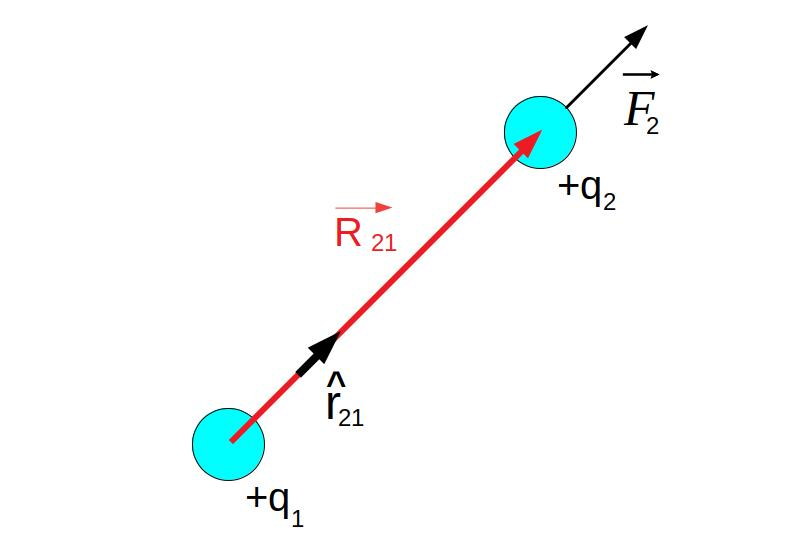
\includegraphics[scale=0.5]{../jpg/Two_Static_ChargesV1.jpg}
\end{center}
\caption{Vector representation of Coulomb's force between two static charges.}
\label{twostaticch}
\end{figure}


\subsection{How perfect is this balance?}




Calculate the repulsive force if there is a little bit of unbalance. Say that each of these two tables in the classroom had 100 extra electrons. Calculate the electrostatic force between the two tables. 















\subsection{Properties of Electric Charge}

\subsubsection{Electric charge cannot be created or destroyed.} 

If the total net charge of an object is $q$, and if that object has $n_e$ electrons and $n_p$ protons, then the total charge is $q=n_p e-n_e e$. 

%{\large EXAMPLE}

%An object has 3 protons and 2 electrons. Find what is the net charge of %the object. Assume that the 2 protons and 2 electrons have recombined %(became neutral). What is the net charge now?

\subsubsection{What is the electric force if we have more than two charges?}

The total electric field at a point in space from the two charges is equal to the sum of the electric fields from the individual charges at that point.

%{\large EXAMPLE} Two positive unit charges are fixed in air in Cartesian %coordinate system at points A(0,-1) and B(0,1). Find the electric field %at the points C(0,0) and D(1,1).

\subsubsection{What if the charge is not in air?} 

Let's look at Coulomb’s law again. 


\begin{eqnarray}
\vec{F_e}=\frac{q_1 q_2}{4 \pi \epsilon_0 r^2} \hat{R_{12}}
\end{eqnarray}\label{Coulombslaw2}
Which quantity in this formula depends on the material? $\epsilon_0$. If the charge is within a dielectric material, then we need to account for that by changing this $\epsilon_0$ somehow. If we place the charge inside a dielectric material what do you think will happen with the atoms in the material? The atoms will get distorted and polarized. Such a polarized atom we call an electric dipole. The distortion process is called polarization. Because the material acts in such a way, the electric field around this point charge is different than if there was no material. In any dielectric medium, the electric field is defined as


\begin{eqnarray}
\vec{F_e}=\frac{q_1 q_2}{4 \pi \epsilon r^2} \hat{R_{12}} \\
\epsilon = \epsilon_0 \epsilon_r
\end{eqnarray}\label{Coulombslaw3}

We added unitless quantity $\epsilon_r$, relative dielectric constant. $\epsilon_r$ values for different materials can be Googled. Some examples of dielectric constants are $\epsilon_r$: air $\epsilon_r$=1,  teflon $\epsilon_r$=2.2, glass $\epsilon_r$=4.4, Silicon $\epsilon_r$= 11, GaAs $\epsilon_r$=12, distilled water $\epsilon_r$= 80. 



\subsection{Principle of Superposition}

If we have two charges, the total field due to both charges is equal to the vector sum of the fields due to individual charges, see Figure \ref{superposition}.  The field at



\begin{figure}[htbp]
\begin{center}
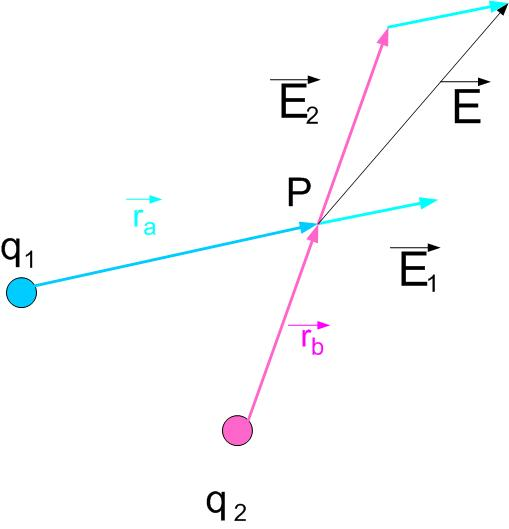
\includegraphics[scale=0.5]{../jpg/superposition.jpg}
\end{center}
\caption{Electric Field due to two charges.}
\label{UnitCh}
\end{figure}

The fields or charges $q_1$ and $q_2$ are:

\begin{eqnarray}
\vec{E_1}=\frac{q_1}{4 \pi \epsilon_{0} {r_a}^2} \hat{r_a} \label{field}\\
\vec{E_2}=\frac{q_1}{4 \pi \epsilon_{0} {r_b}^2} \hat{r_b}
\end{eqnarray}

Where $\hat{r_a}$ and $\hat{r_b}$ are unit vectors in the direction of $r_a$ and $r_b$. The total field due to both charges is


\begin{eqnarray}
\vec{E}=\vec{E_1} + \vec{E_2} 
\end{eqnarray}






\subsection{Electric Force in Rectangular Coordinates}


In general equation for the electric force is given as



\begin{eqnarray}
\vec{F}=\frac{q_1 q_2}{4 \pi \epsilon_{0} {r_a}^2} \hat{r_a} \label{genfield}
\end{eqnarray}

The electric field at a point $P(x,y,z)$ due to a charge $q_1$ positioned at a point $P_{q_1}(x_1, y_1, z_1 )$  in the rectangular coordinate system is shown in Figure \ref{singlecharge}. The position vector of the point $P_{q_1}$  is 


\begin{figure}[htbp]
\begin{center}
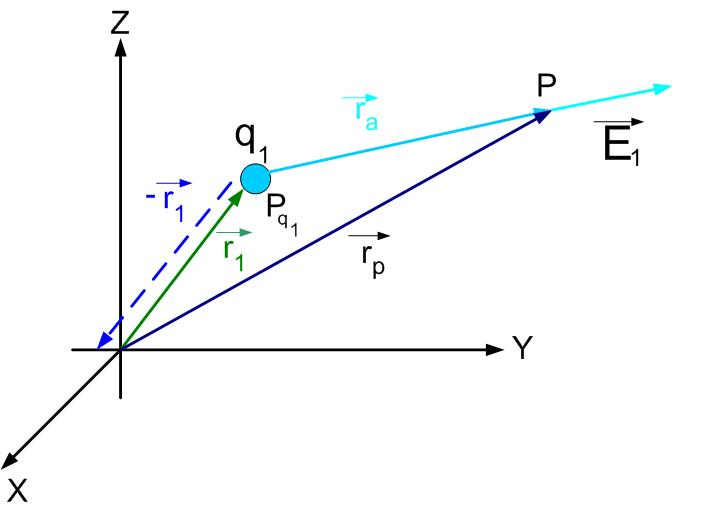
\includegraphics[scale=0.5]{../jpg/singlechargecartcoord.jpg}
\end{center}
\caption{Electric Field due to a unit charge in Rectangular coordinate system.}
\label{singlecharge}
\end{figure}





\begin{eqnarray}
\vec{r_1}=x_1 \vec{x} + y_1 \vec{y} +z_1 \vec{z}
\end{eqnarray}

The position vector of point $P$ is equal to

\begin{eqnarray}
\vec{r_p}=x\vec{x} + y \vec{y} +z \vec{z}
\end{eqnarray}

The two vectors mark the beginning and the end of the distance vector $\vec{r_a}$  between points $P_{q_1}$ and $P$. The vector  $\vec{r_a}$ is the sum of vectors $-\vec{r_p}$ and $\vec{r_1}$



\begin{eqnarray}
\vec{r_a}=\vec{r_p} + (-\vec{r_1})
\end{eqnarray}

When we substitute position vectors $r_1$ and $r_p$:

\begin{eqnarray}
\vec{r_a}= (x - x_1) \vec{x} +(y - y_1) \vec{y} +(z - z_1) \vec{z}
\end{eqnarray}

Vector $\vec{r_a}$ has the magnitude of:


\begin{eqnarray}
|\vec{r_a}|= \sqrt{(x - x_1)^2 +(y - y_1)^2 +(z - z_1)^2}
\end{eqnarray}

Unit vector in the direction of vector $\vec{r_a}$ is:


\begin{eqnarray}
\hat{r_a}= \frac{\vec{r_a}}{|\vec{r_a}|} \\
\hat{r_a}=\frac{\vec{r_a}}{\sqrt{(x - x_1)^2 +(y - y_1)^2 +(z - z_1)^2}}
\end{eqnarray}



\begin{eqnarray}
\vec{E_1}=\frac{q_1}{4 \pi \epsilon_{0} {r_a}^2} \hat{r_a}
\end{eqnarray}

Where $r_a$ is the distance between the charge $q_1$ and the point $P$. Substituting expressions for $\hat{r_a}$, and $|\vec{r_a}|$ in equation \ref{genfield} we get

 



\begin{eqnarray}
\vec{E_1}=\frac{q_1}{4 \pi \epsilon_{0} {\sqrt{(x - x_1)^2 +(y - y_1)^2 +(z - z_1)^2}
}^3} \vec{r_a} \label{eqonecharge}
\end{eqnarray}

Substituting 


For two charges, as shown in Figure \ref{twocharges} equation \ref{eqonecharge} becomes

\begin{eqnarray}
\vec{E}= \frac{q_1}{4 \pi \epsilon_{0} {\sqrt{(x - x_1)^2 +(y - y_1)^2 +(z - z_1)^2}
}^3} \vec{r_a} + \frac{q_2}{4 \pi \epsilon_{0} {\sqrt{(x - x_2)^2 +(y - y_2)^2 +(z - z_2)^2}
}^3} \vec{r_b} 
\end{eqnarray}


\begin{figure}[htbp]
\begin{center}
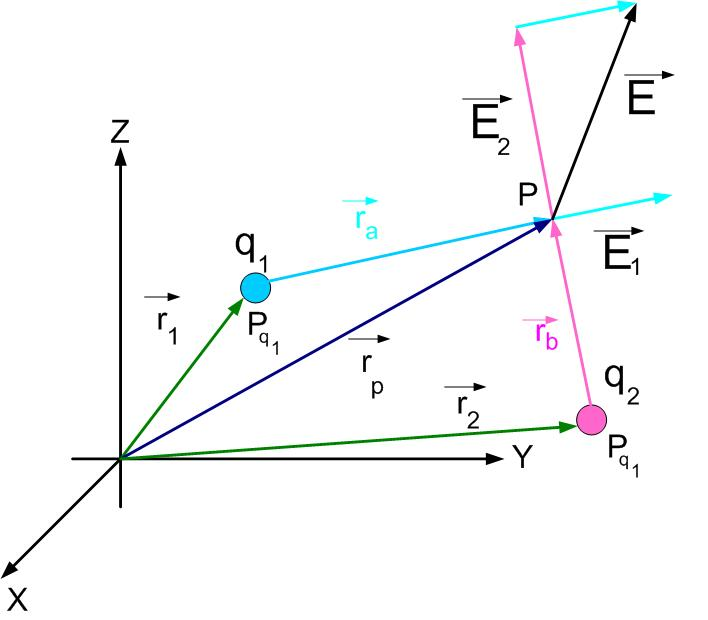
\includegraphics[scale=0.5]{../jpg/twochargescartcoord.jpg}
\end{center}
\caption{Electric field due to two charges in  Rectangular coordinate system.}
\label{singlecharge}
\end{figure}






\end{document}